\spaltenanfang


\abschnitt{Zusammenfassung \& Abenteuerverlauf}

Die Eruption der \textbf{Silberkrone} hat Ende 1039 BF den Vulkanismus im \textbf{Rorwhed} wieder geweckt.
Ausgelöst wurde sie durch ein Ritual des Tairach-Priesters Gushrogh Drughai.
Die örtlichen Hexen verloren als Folge ihren Tanzplatz, doch auch die Bewohner der Umgebung sind seitdem von den Auswirkungen betroffen.
Die Eruption beschädigte auch das magische Geflecht, welches an diesem Ort besonders intensiv auftritt:
Kraftlinien und Feenpfade sind in Unordnung oder zerrissen und ihre Kraft fließt ins Diesseits.
Über die Feenpfade tauchen manche merkwürdigen Kreaturen auf und sorgen für Unruhe in der Umgebung.


Besonders hart getroffen hat es die örtliche Dryade Venaya:
Sie wacht seit Jahren über ein Tal im Schatten des Gipfels.
Doch seit der Schamane sie gezwungen hat, an seinem Ritual teilzuhaben, leidet sie unter einer permanenten Verbindung zu Tairachs Geisterwelt, welche jede Nacht droht, aktiv zu werden.
Zudem ist sie als Dryade auch mit ihrem Baum durch ein magisches Band fest verbunden und müsste dadurch eigentlich immer vom Schwelbrand betroffen sein, der dessen Wurzeln versengt.
Nur weil sie ein Wesen des Humus ist, regeneriert sie mit ganz besonderer Geschwindigkeit, sodass ihr des Tags wenig anzumerken ist.
Doch in vielen Nächten wird sie Opfer einer Besessenheit, sodass die Regeneration nicht funktioniert -- die Lebenskraft geht stattdessen direkt an Tairach.
Ab da erleidet sie die vollen Auswirkungen des Schwelbrandes an ihrem Baum und wird zu einem rasenden Wesen aus Qualm.
In diesem Zustand zieht sie durch die Lüfte und fährt auf nichtsahnende Bewohner des Svelltlandes herab.

\vfill

Spätestens zum Morgengrauen würde die Besessenheit enden, doch oft ist Venaya vorher schon zerfallen und liegt als schnell neu keimender Schössling in ihrer eigenen Asche.
Sie kehrt zu ihrem Tal zurück und hat nur wirre Erinnerungen an eine wüste graue Ebene.
Das herauszufinden und eine Lösung zu finden soll die wichtigste Aufgabe der Helden in diesem Abenteuer sein.
Dazu reist die Gruppe von \textbf{Lowangen} aus durchs Svellttal ins Rorwhed-Gebirge.
Zu Beginn können sie zwischen der Route über \textbf{Arsingen} und der über \textbf{Ansvell} wählen, danach führt die Straße durch \textbf{Svellmia}, die Ruinen von \textbf{Tiefhusen} und über \textbf{Rorkvell} ins Gebirge.

\neuespalte

\abschnitt{Einstiege Spielercharaktere}
Die hier vorgestellten Einstiege bieten eine Möglichkeit, wie die verschiedenen Charaktere in das Abenteuer starten und welche Motivation sie haben können, um die Reise anzutreten.
Sie sind aber nicht verpflichtend.
Sollten die Spielleiterin oder die Spieler weitere Ideen haben, können sie diese gerne hinzufügen.


\absatz{Charaktere, die einfaches Geld suchen und sich verteidigen können}
\textbf{Vanjescha Stoerrebrandt}, Leiterin des Kontors in \textbf{Tjolmar}, plant den Ausbau der Handelsstraße von Tjolmar nach \textbf{Riva}.
Ihr Sekretär \textbf{Valpo Lucianus von Sturzbach} hat dafür vom Kontor in Lowangen eine Lieferung topographischer Geräte und eine Projektkasse mit 5.000 Dukaten für diverse Lohnarbeiten entgegengenommen und benötigt nun eine Eskorte.

\absatz{Charaktere mit hohem Sozialstatus}
Die Sprengung der Silberkrone, eines Berges im Rorwhed-Gebirge, durch ein Ritual eines orkischen Tairach-Schamanen sorgt für Unruhe unter den Führungskräften eurer Institution.
Euer Vorgesetzter hat euch losgesandt, um einen versiegelten Brief an \textbf{Barngrimm Radobrecht}, den Großmeister des \textbf{Ordens der Grauen Stäbe} in Lowangen persönlich zu übergeben.

\absatz{Naturverbundene Charaktere}
Euer Weg hat euch schon vor einer Weile nach \textbf{Lowangen} geführt.
Zunächst angewidert von der lauten und engen Stadt habt ihr aber schon bald euren Platz als Beschützer und Heiler der wehrlosesten Bewohner gefunden: der Tiere.
Zuletzt häufen sich aber verletzte Wildtiere unter euren Patienten, die im Norden der Stadt mit bereits älteren Verbrennungen gefunden werden.
Einige der Städter erzählten euch von einem Vulkan, der die Natur in seiner Umgebung verwüstet.


\absatz{Naturverbundene Magiebegabte}
Euer Zirkel hat von der Sprengung der Silberkrone und der Vernichtung des Tanzplatzes des örtlichen Hexenzirkels durch den orkische Tairach-Priester \textbf{Gushrogh Drughai} erfahren.
Eurer Anführer hat euch daraufhin losgesandt, um Hilfe anzubieten.
Zwar herrscht in der Region inzwischen Frieden zwischen Menschen und Orks und sogar eine vorsichtige Annäherung --
allerdings sind besonders die lokalen Hexen noch skeptisch, ob dies auch für sie gilt.

\absatz{Charaktere mit niedrigem Sozialstatus und Bedarf an Geld}
Das Leben während der Belagerung der Drughash-Orks (1031 BF) war für alle hart.
Während der Adel auf seine sogenannte Ehre geachtet hat, hattet ihr nicht die Möglichkeiten für solchen Luxus.
Also habt ihr für freies Geleit wichtiger Waren in die Stadt, manchen Ork mit Informationen über die Verteidigung versorgt.
Dabei habt ihr gute Kontakten mit diesen geknüpft.
Leider haben einige der \enquote{aufrechten} Verteidiger von damals davon erfahren und wollen Rache nehmen, weswegen es günstig wäre zu verschwinden.
In den Kneipen hört ihr Gerüchte über eine hohe Belohnung von der Torf-Compagnie für die Ergreifung von -- wandernden Wildschweinfässern?

\spaltenende

\absatz{Welcher Held weiß von welchen Ereignissen?}

\tabelle{lXXXXX}{
& Ascheregen, verletzte Tiere & Stoerrebrandt-Lieferung & Brief an den Großmeister & Hexen im Rorwhed & Wildschwein\-fässer \\
Streuner &   & x &   &   & x \\
Hexe     & x &   &   & x &   \\
Druide   & x &   &   & x &   \\
Geweihte & x &   & x &   &   \\
Kriegerin &  & x & x &   & x \\
}

\spaltenanfang


\abschnitt{Begegnungen Lowangen}

Die freie Stadt \textbf{Lowangen} ist der größte Handelsknotenpunkt im Norden.
Nach Jahren des Widerstandes gegen die orkische Expansion, zuletzt bei der Belagerung der Stadt durch die Drughash-Orks 1031 BF ist man inzwischen zu einer Übereinkunft gekommen, in der zweimal im Jahr ein Tribut an die Schwarzpelze entrichtet wird, die ohnehin inzwischen das Umland kontrollieren.
Dafür konnte die Stadt ansonsten ihre alten Rechte behalten, beispielsweise wählt der Gildenrat weiterhin den Bürgermeister.
Auch der \textbf{Lowanger Dualismus}, eine sektenartige Ausprägung des Zwölfgötterglaubens, in dem Praios als der Gott allen Glücks und Boron als das Böse betrachtet wird, ist weiterhin lebendig, wenn auch die Annäherung an die Orks eine Herausforderung für seine sittenstrengen Gläubigen darstellt.


Die Stadt teilt sich in drei Viertel auf. Auf einer Insel im Svellt liegt das reiche \textbf{Alt-Lowangen}, welches das Zentrum der Stadtverwaltung und des Handels darstellt. Im Norden am Flussufer liegt die \textbf{\enquote{Bunte Flucht}}, ein Künstlerviertel mit einigen zugezogenen Elfen und vielen Tempeln.
Südlich davon liegt \textbf{Eydal}, ein ehemaliges Dorf, das sich widerwillig aufgrund der Orküberfälle hat eingemeinden lassen.
Das Bild ist geprägt von zwergischen Ursprüngen und dem Ingerimm-Tempel.
(Mehr dazu in \emph{Reich des Roten Mondes:65--73} (Tabelle mit Unterkünften S.\,69).)


\absatz{Kontor Stoerrebrandt (Alt-Lowangen)}
Das Kontor ist kein Ort der Ruhe:
Überall stehen Kisten und eilen Angestellte von Flur zu Flur. In einem edlen Büro im ersten Stock erledigt der diensteifrige Sekretär \textbf{Valpo Lucianus von Sturzbach} noch einige bürokratische Feinheiten, bevor er mit einer Eskorte aufbricht,
	um seiner Herrin \textbf{Vanjescha Stoerrebrandt} im Tjolmarer Kontor die benötigten Utensilien und Finanzen für ihr großes Herzensprojekt liefert:
	Der Ausbau der Handelsstraße von \textbf{Tjolmar} nach \textbf{Riva}.
	Er hat bereits zwei Haudegen angeworben, allerdings würde er sich angesichts des Wertes seiner Ladung über weitere Söldner freuen, die ihn zumindest einen Teil des Weges begleiten. 
	er Tageslohn dafür beträgt 4~Silber. Zunächst gilt es aber, die letzten Versicherungen abzuzeichnen, sollte es zu spontanen Tributforderungen oder Zollsperren durch orkische Truppen kommen.


\absatz{Im Ordenshaus der Grauen Stäbe (Bunte Flucht)}
Im Ordenshaus herrscht unruhiges Geflüster: \textbf{Magistra major Vistella Jolen} ist vor einer Woche mit bleichem Gesicht und seltsamen Neuigkeiten von einer Reise nach \textbf{Tjolmar} zurückgekehrt. So habe südlich des \textbf{Rorwhed}s ein seltsamer Ascheregen in der Luft gehangen, der sich, nach einer \textsc{Oculus Astralis}-Analyse als magisch herausgestellt hat \emph{(Ilaris:80,141)}.
Irritiert von ihrer Entdeckung legte sie eine \emph{Sinnenschärfeprobe} nach, um eine \emph{Strukturanalyse} \emph{(Ilaris:80)} durchzuführen. Das wirre Muster der Kraftfäden habe sie an den Rande der Erschöpfung getrieben, doch mit Mühe konnte sie eine Sache erkennen: Es handelt sich um die Spur eines feenartigen Wesens, dessen urtümliche Magie von inneren Bränden verzehrt wird.

Nun sammelt der Orden eine Investigativ-Gruppe, die diese Beobachtung untersuchen soll.
Sollte sich unter den Heldinnen eine Person mit magischem Wissen und passendem Sozialstatus befinden, wird \textbf{Großmeister Barngrimm Radobrecht} ihm einen Platz anbieten, oder diese als Vorhut vorausschicken.


\absatz{\enquote{Bestraft die Spitzel!}}
Die Helden biegen in eine Straße ein und sehen eine Gruppe von vier Personen (Werte im Anhang unter Banditen), die auf eine liegende Person eintreten.
Sie können helfen: Mit einer \emph{Laufen}-Probe (Schwierigkeit 14) wäre das Opfer in der Lage zu fliehen. Die Gruppe könnte die Angreifer einschüchtern und damit eine Erleichterung von +4 für die Probe des Opfers generieren, oder sie lenken sie mit Taschenspielertricks ab (+2).

Bei dem Opfer handelt es sich wie eventuell bei einem der Helden um einen ehemaligen Schmuggler und Spitzel, der den Orks 1031 BF wertvolle Informationen über die Verteidigung der Stadt hat zukommen lassen. Seine Angreifer sind ehemalige Mitglieder der Stadtmiliz, die die \enquote{Verräter an der Stadt und der Freiheit} bestrafen wollen.

\newpage

\abschnitt{Reisen im Svellt}
Hier werden ein paar mögliche Begegnungen beschrieben, die die Helden haben können. Im \ref{svellt}{Anhang} finden sich zudem kurze Auflistungen von Tieren und Pflanzen der Region. Auf jeden Fall sollte die Gruppe Hinweise auf den \textbf{Qualmgeist} erhalten und ihm vielleicht selbst schon gegenübertreten müssen.

Jagdregeln finden sich \emph{Ilaris:68}. Die Basis bilden dabei Proben auf \emph{Überleben}.
Das Svelltland kann hierfür als \emph{wildreich} gelten, die Schwierigkeit liegt also nur bei 12.

(Wesentlich ausführlichere Listen von Tieren: \emph{Zoo-Botanica:277--280}.)

Die meiste Zeit wird die Gruppe Gewässer in der Nähe haben, zu Beginn die sumpfigen Gegenden zwischen \textbf{Lowangen} und \textbf{Svellmia},
dazu den \textbf{Lowanger Svellt} oder den \textbf{Svall}, die alle früher oder später in den großen Flusslauf münden.
Diesen Umstand könnten die Helden nutzen, um nach Kräutern zu suchen, die nur in entsprechend feuchten Umgebungen wachsen, doch könnten sie dort auch auf ungewöhnliche Gegner treffen wie \textbf{Riesenamöben} (Werte im Anhang).

\absatz{Begegnungen auf und abseits der Straße}
\begin{itemize}
\item An einem Stadttor diskutiert ein verzweifelt aussehender Schneider mit den \textbf{Torwachen}, einem Ork und einem Menschen. Für seine Stoffe und Tücher soll er Abgaben zahlen, er selbst spricht jedoch von „Wegelagerei“.

\item Zwei Orks kommen euch auf dem Pfad entgegen. Bögen, befüllte Köcher und Jagdmesser im Gürtel weisen sie als \textbf{Jäger} aus. Auf ihrem Karren liegt ein stattlicher Sechsender.

\item Am Wegesrand spielen ein paar Kinder den Fall \textbf{Tiefhusen}s nach. Die meisten haben sich die Gesichter bemalt und brüllen in einem Mischmasch aus orkischen, menschlichen und zwergischen Wörtern. Bei zweien artet das Spiel in eine wilde Prügelei aus.

\item Zwergin \textbf{Bischa, Zahnreißer Dollinger} und \textbf{Maultier Atze} reisen die Straße entlang Richtung Praios. Dollinger verspricht eine „unglaublich billige und fast schmerzfreie Zahnbehandlung, najaa, vermutlich.“

\item Die Geräusche verraten es -- durchs Halbdickicht eines bewaldeten Hangs brechen große Tiere.
Dann kommen sie in Sicht und überraschenderweise sind es \textbf{Weinfässer}, denen metallene Beine und Köpfe gewachsen sind, sodass sie wirken wie größere Wildschweine.
Ihnen auf den Fersen ist eine Rotte \textbf{Goblin}s auf echten Schweinen; einem gelingt es, auf ein Fass zu springen und sich festzuhalten.

\item Aus einem Gehöft kommen drei stämmige \textbf{Ork}s.
Die vorderen beiden haben je eine Ziege unter den Arm geklemmt, der hinterste notiert etwas auf einer kleinen Wachstafel.
Die wettergegerbte Bäuerin schaut ihnen auf eine Forke gestützt hinterher.

\item Am Waldrand liegt das Nachtlager einer \textbf{Reisegruppe}, welche überstürzt aufbrechen musste.
Gepäck und Schlafsäcke liegen noch da, sind aber von Ruß und Asche bedeckt oder halb verbrannt.
Auch in der Umgebung finden sich Brandspuren an Bäumen und verschweltes Gras. 
\end{itemize}

Vielleicht suchen die Helden die weitere Umgebung ab oder fragen in der nächsten Ortschaft, dann können sie mit einem Augenzeugen sprechen \emph{(Quelle 1 im Anhang auf S.\,\pageref{aiw_quelle1})}.
Später auf der Reise kann ein abgebranntes Gehöft die gleichen Spuren aufweisen, die Bauersleute kamen mit dem Leben davon.


\probenkasten[bild=ueberleben,
zusammenarbeit=nein,
gruppenprobe=gut,
pw=12,
farbe=gruen,
erfolg={},
misserfolg={}
]{Fährtensuchen (Überleben), Sinnenschärfe (Wahrnehmung)}
{\emph{Recherche:} Was ist hier geschehen? (Rechercheregeln \emph{Ilaris:69}, Dauer: halbe Stunde)\\
Anhand der Spuren um das Gehöft herum lassen sich Schlussfolgerungen über mögliche Angreifer ziehen.

\textbf{IG 1:} Hier war etwas, das geglüht haben muss. In einem großen Kreis um die Szene herum ziehen sich Spuren von Asche und verkohlter Vegetation.\\
\textbf{IG 2:} An Bäumen in der Nähe sind Nadeln oder Blätter versengt, hier kam der Angreifer offenbar durch die Baumwipfel direkt vom Himmel herab.\\
\textbf{IG 3:} Die Spuren weisen weniger auf einen Drachen hin, eher auf eine Art Feuerwesen, ein Elementar oder Dämon vielleicht, doch die magischen Spuren sind bereits verflogen.
}

\vfill

\absatz{Der Qualmgeist}
Die Helden können auf der Reise auch selbst schon mit dem \textbf{Qualmgeist} Bekanntschaft machen.
Er wird in den meisten Nächten aktiv (1--4 auf W6) und lässt sich vom Wind ins Land tragen.
Hat er Opfer ausgemacht, fährt er vom Nachthimmel auf sie herab, umkreist die Gegner und bewirft sie mit Feuerzaubern.
Die Helden können ihn töten, ohne das Finale in Gefahr zu bringen (Kampfwerte und eine detailliertere Beschreibung auf S.\,\pageref{geist}).

Noch ahnen nur die Hexen, dass die \textbf{Dryade} aus dem \textbf{Rorwhed} dahintersteckt.

\newpage

\absatz{Die Weinlegende}
Auf der Reise bietet sich an, in einer prall gefüllten Taverne den alten \textbf{Strupp} die Legende von Jokmanns Wein erzählen zu lassen (Quelle~2 auf S.\,\pageref{aiw_quelle2} im Anhang).
Das bereitet die Begegnung mit den Goblins vor, außerdem unterhalten sich die Gäste auch über die gesichteten Wildschweinfässer, was Helden, die auf dieser Fährte sind, interessieren könnte.

Möglich sind hier folgende \emph{Ermittlungen} und \emph{Recherchen}:
\probenkasten[bild=beeinflussung,
zusammenarbeit=nein,
gruppenprobe=gut,
pw=14,
farbe=gruen,
erfolg={},
misserfolg={}
]{Überreden, Betören, Belauschen (Heimlichkeit), Menschenkenntnis}{
\emph{Recherche:} Das Geheimnis von \textbf{Jokmann}s Wein (Dauer: 3 Stunden;
Unterstützung: Von Sturzbach (+4), Berufung auf naturnahe Götter (+2))\\
Einige weitere ältere Gasthausbesucher kannten den alten \textbf{Jokmann} ebenfalls und haben seine legendäre Weinkaraffe gesehen. 

\textbf{IG 1:} Die Figuren auf der Karaffe waren klein und rot  -- manche ritten auf Schweinen.\\
\textbf{IG 2:} In der Nähe von Jokmanns Revier wurden immer mal wieder Goblins gesichtet.\\
\textbf{IG 3:} Zwischen Rorwhed und Odenmoor lebt eine Goblinsippe, die von einer zaubermächtigen Schamanin angeführt wird.\\
\textbf{IG 4:} Nach langen Nachfragen durch die Helden wird sich Strupp erinnern, dass er gesehen hat, wie Jokmann sich im Wald manchmal mit Goblins unterhalten hat.
}

\probenkasten[bild=magiekunde,
zusammenarbeit=nein,
gruppenprobe=gut,
pw=15,
farbe=blau,
]{Feenmagie (Magiekunde), Jagen (Überleben), Überreden, Betören, Belauschen (Heimlichkeit)}
{
\emph{Ermittlung:} Wo sind die Wildschweinfässer? (Dauer: 2 Stunden;
Unterstützung: Von Sturzbach (+2), Lokalrunde für 2 Silber (+4))
Viele der anwesenden Besucher haben die Fässer in der Nähe des \textbf{Rorwhed}s gesehen, wo diese etwas zu suchen schienen.
}

\probenkasten[bild=magiekunde,
zusammenarbeit=ja,
gruppenprobe=gut,
pw=20,
farbe=blau,
]{Elementarmagie (Magiekunde), Wetterkunde (Überleben), Überreden, Betören, Belauschen (Heimlichkeit)}
{
Recherche: Geschichten über den \textbf{Qualmgeist} (Dauer: 5 Stunden;
Unterstützung: Autorität der Ordnungshüter ( Berufung auf Auftrag des ODL oder eines Tempels oder Verweis auf Gruppenmitglieder) (+4), Freibier (+2))

Manche Besucher haben die Spuren des mysteriösen \textbf{Qualmgeist} gesehen. Sie könnten Hinweise auf dessen Ursprung geben.

\textbf{IG 1:} Meistens wurden verbrannte Stellen oder Gebäude gefunden, nachdem in der Nacht zuvor einen seltsamen Ascheregen beobachtet wurde.\\
\textbf{IG 2:} Der Ascheregen taucht häufig auf, wenn der Wind in der Nacht aus dem Rorwhed kommt.\\
\textbf{IG 3:} Es ist eine Gestalt im Innern des Rauchs zu sehen, die nach einigen Stunden zu Asche zerfällt.\\
\textbf{IG 4:} In der Asche findet sich das Samenkorn einer Esche.
}

\newpage

\absatz{Goblins}
Die Goblinsippe unter der Führung ihrer Schamanin \textbf{Aschka der Verhüllten} siedelt seit Jahrhunderten in der Region zwischen dem Rorwhed und dem Odenmoor.
Allerdings ist es nicht der Wein, der das Jagdglück bringt, sondern die Karaffe, aus der er getrunken wird.
Denn auf dieser liegt ein \textsc{Adlerauge Luchsenohr}  \emph{(Ilaris:130}, der die Wahrnehmung der Jäger erhöht.
Wenn die Helden ein Lager der Goblins betreten, werden sie einige aufgeregte Jagdgruppen treffen, die sich ebenfalls für die Jagd auf die Wildschweinfässern vorbereiten.
Diese sind aber nicht auf die Belohnung der Torf-Compagnie aus, sondern sehen in der tierischen Form der Fässer ein Geschenk \textbf{Mailam Rekdai}s an ihre Kinder.

Sollte die Gruppe sich nach dem Ascheregen oder ähnlich komplexen Themen erkundigen, werden sie an die Schamanin \textbf{Aschka} weitergeleitet.
Bezüglich des Qualmgeistes wird sie den Helden erklären, dass sie in ihrer Meditation ein Feuer in der Erde verspürt hat, dass, als sie es näher betrachten wollte, ebenfalls angefangen hat, an ihrem Astralleib zu zehren.
Sie vermutet, dass die Hexen mehr wissen, zumindest wirkten diese bei Begegnungen zuletzt äußerst unstet.

\probe{beeinflussung}{Überreden (16)}{
Das Geheimnis des Weins wird sie den Helden nur mit einer gelungenen Probe verraten.
Nur mit einer zweiten Überredenprobe (Schwierigkeit 20) wird sie ihnen eine Karaffe übergeben.
}

\neuespalte

\absatz{Hexen im Rorwhed}
Im \textbf{Svelltal} gibt es mehrere \textbf{Hexenzirkel}. Der mächtigste davon ist der Zirkel im \textbf{Rorwhed}, der von der Oberhexe \textbf{Xerinn} angeführt wird.
Ein weiterer ist der des \textbf{Grauen Wald}es unter dem Oberhexer \textbf{Bringimox}.
Der \textbf{Graue Wald} hat den Hexen vom \textbf{Rorwhed} nach der Sprengung Asyl gewährt, was zu einer tiefen Freundschaft zwischen den Zirkeln geführt hat.
Die aufbrausende Katzenhexe \textbf{Xerinn} kämpft allerdings weiterhin mit der fulminanten Niederlage, die die Zerstörung des Tanzplatzes für ihre Pläne hinsichtlich der Macht im \textbf{Rorwhed} bedeutet.
Denn statt den Widerstand gegen die Orks weiterzuführen, muss sie nun sehen, wie sie Auflösung ihres eigenen Zirkels verhindert.

Der Eulenhexer \textbf{Bringimox} sorgt sich dagegen mehr um das Loch in den Feenpfaden.
Als die beiden Anführer die Umgebung des Berges untersucht haben, haben sie den glühenden Dryadenbaum gefunden und konnten sich angesichts der Berichte über die brennenden Höfe und den Qualmgeist zusammenreimen, wie diese beiden Dinge zusammenhängen.
Sie sehen die Lösung in der Heilung des Baumes, wozu sie aber ausgewählte Leute aus beiden Zirkeln mit in das Tal der Dryade bringen müssen, die mit ihnen zusammen die Kraftfäden der Feenpfade wieder zusammenflicken und den magischen Brand in den Wurzeln des Baumes löschen.

Bisher sind sie noch nicht zur Tat geschritten, weil dieses Ritual zeitintensiv ist und sehr schmerzhaft für die Dryade sein wird.
Beide fürchten, dass der anhaltende Schmerz die Dryade zur Verwandlung zwingen wird, was ein lebensgefährliches Risiko für die Ritualteilnehmer darstellt.
Beide möchten aber auch, dass diese Angelegenheit von den Hexen selbst geregelt wird.

Sollten die Helden den Zirkeln von der inzwischen bereits aufgebrochenen Untersuchungseinheit der \textbf{Grauen Stäbe} berichten, werden sich die beiden Oberhexen zum Handeln gezwungen sehen.

\spaltenende

\newpage
\spaltenanfang
\abschnitt{Finale im Tal der Dryade}
Die Hexen bereiten sich auf das Ritual vor, welches eine Stunde vor Mitternacht beginnen und die Kraftlinien und Feenpfade schließen soll.
Während sie es vollziehen, müssen sie durch der Heldengruppe geschützt werden vor den Angriffen des \textbf{Qualmgeist}es.
Falls es der Gruppe nicht schon klar ist, wissen \textbf{Bringimox} oder \textbf{Xerinn} zu berichten,
dass die \textbf{Dryade} des Tals identisch ist zu dem \textbf{Qualmgeist}, der des nachts umgeht.


Die Helden könnten auf die Idee kommen, mit der \textbf{Dryade} zu sprechen.
Sie hält sich tagsüber immer in ihrem Tal auf.
Es ist durchzogen von einem warmen, brenzligen Geruch.
Hier sind manche Büsche und Bäume noch grün und frisch, andere verkohlt, dazwischen stecken Felsbrocken, Überbleibsel der Detonation der Bergspitze.
Dazwischen steht einzeln der noch lebende, aber teils geschwärzte Baum der Dryade.
Vom Ritual rühren die langen Nägel, die in den Stamm eingeschlagen sind und ein großer, rot eingefärbter Stierschädel über einem Ast.

Wenn die Helden sich den Baum ansehen, erscheint sie:
Etwas größer als ein Mensch, so grün belaubt und schön wie es Dryaden eigen ist, aber auch müde und mit Ruß und Asche verschmiert.
Während des Gesprächs schließen sich verkohlte Stellen, doch anderswo stiebt erneut Asche auf.


Sie weiß um ihre Verwundung, aber erinnert sich nur verschwommen an die Nächte der letzten Wochen.
Auf jeden Fall macht sie den Helden klar, dass sie für nichts garantieren kann, sobald die Dunkelheit hereinbricht:
Ihre Qualmgestalt erscheint etwa zum Licht der ersten Sterne und dann hat sie keinerlei Kontrolle mehr.
Bis dahin können die Helden versuchen, den Hexen bei den Vorbereitungen zu helfen.


Wenn die Nacht hereinbricht, beginnt \textbf{Venaya} immer stärker zu qualmen.
Meist beginnt kurz danach eine Besessenheit, denn für die Geister ist sie in diesem Zustand ein offenstehendes Tor.
Wenn das geschieht, erhebt sie sich meist mit einem \textsc{Leib des Windes} \emph{(Ilaris:147f.)} in die Lüfte und lässt sich vom Wind weit ins Land tragen, um wahllos Gehöfte oder Reisende anzugreifen.


In Verteidigung gegen den Qualmgeist können die Helden auf einen schnellen Sieg im Kampf setzen.
Wenn sie besiegt wird, zerfällt sie zu Asche, unter welcher sie als Sprössling bis zum Morgengrauen neu heranwächst.

Oder sie können Magie einsetzen, um sie sich und den Hexen vom Leib zu halten:
\textsc{Einfluss}zauber \emph(Ilaris:133--136) könnten sie auf Abstand halten, mit einem \textsc{Harmoniesegen} \emph{(Ilaris:177)} wäre sie für eine Weile besänftigt, ein \textsc{Geisterbann} \emph{(Ilaris:166)} könnte sie wieder in ihr natürliches Wesen zurückfinden lassen -- kreative Einfälle sollten belohnt werden.

Das Ritual der Hexen dauert etwa zwei Stunden. Sobald dieses abgeschlossen wurde, hebt sich ein Windhauch durchs Tal, schüttelt kräftig die Baumkronen durch und die wilden Magieströme finden zu einer Ordnung zurück.
Die Verbindung der \textbf{Dryade} zu \textbf{Tairach}s Geisterwelt reißt ab und die Wunden im Tal können heilen.

\kreatur{Qualmgeist}{Ein Qualmgeist}{elementar}{
	\label{geist}
    \kreaturkampfwerte{8}{6}{5}{4}
    \trennlinie
    \kreaturvorteile{
        Aura (Hitze, Zähigkeit (20) alle 4 Initiativephasen, 1 Wunde), Immunität (Feuer), Verwundbarkeit I (Wasser), Flammenkörper (Alle Waffen, die Holz beinhalten, gelten gegen den Qualmgeist als Zerbrechlich (S. 47).}
    \trennlinie
    \kreaturwaffe{Feuerpranken}{1}{10}{16}{2W6+2}{Nachbrennen}
    \kreaturkampfvorteile{Zusätzliche Attacke I}
    \trennlinie
    \kreaturinfo{AsP}{64}
    \kreaturinfo{Feuer}{12 (Brenne, Caldofrigo, Leib des Feuers, Wand aus Flammen, Warmes Blut, Zorn der Elemente)}
    \kreaturinfo{Luft}{10 (Aerofugo, Leib des Windes, Nebelwand, Tlalucs Odem (Qualm statt Gestank), Zorn der Elemente)}
    \kreaturinfo{Eigenschaften}{8 (Atemnot)}
    \trennlinie
    \kreaturinfo{Beschreibung und Verhalten}{In ihrer nächtlichen Form ist die Dryade stark vom Vulkanismus gezeichnet, dessen Glut an den Wurzeln ihres Baumes nagt. Ihre feingliedrige Gestalt verkohlt und wird umhüllt von einer dichten Qualmwolke, die die Nacht noch mehr verdunkelt und auf Mensch und Tiere hustenreizend und erstickend wirken kann. Sie hat keinen Zugriff mehr auf das Element Humus, sondern wirkt Zauber aus den Bereichen Feuer und Luft, um Unbelebtes in Brand zu setzen und Lebewesen zu ersticken.}
}

\vfill

\abschnitt{Der Mühen Lohn}

Nach Abschluss des Rituals bekommt jeder Held 30~EP.
Wenn die Gruppe ihre Verletzungen noch nicht selbst behandelt hat, werden sich die \textbf{Hexen} der beiden Zirkel darum kümmern.
Sie veranstalten außerdem eine schnelle Kollekte, bei welcher 20~Silber als Belohnung für die Gruppe herauskommen -- wenn die Helden noch Auftraggeber aus \textbf{Lowangen} mit ihrer Arbeit und ihren Ergebnissen zufriedenstellen konnten, lassen sich dort auch noch höhere Summen einstreichen. 

Hexer \textbf{Bringimox} drückt einem der Helden noch etwas in die Hand:
Ein Vogelknochen, auf welchem ein Zauber liegt. Zerbricht man ihn, löst das einmalig einen \textsc{Krähenruf} aus \emph{(Ilaris:134)}.
Die \textbf{Dryade} kann zudem anbieten, von der Gruppe gesammelte Kräuter zu verzaubern, sodass sie lange frisch bleiben.

\neueseite

\abschnitt{Anhang}
\absatz{Karte des Svelltlands}
\spaltenende
Eine fangemachte Karte des Svelltlandes findet sich im Blog von telling auf \href{https://tellingaventurien.home.blog/2023/02/27/karte-svelltland-um-1045-nach-bosparans-fall/}{\textbf{\enquote{Zwischen Tisch und Telling}}}. Mit freundlicher Genehmigung des Autors:

\begin{center}
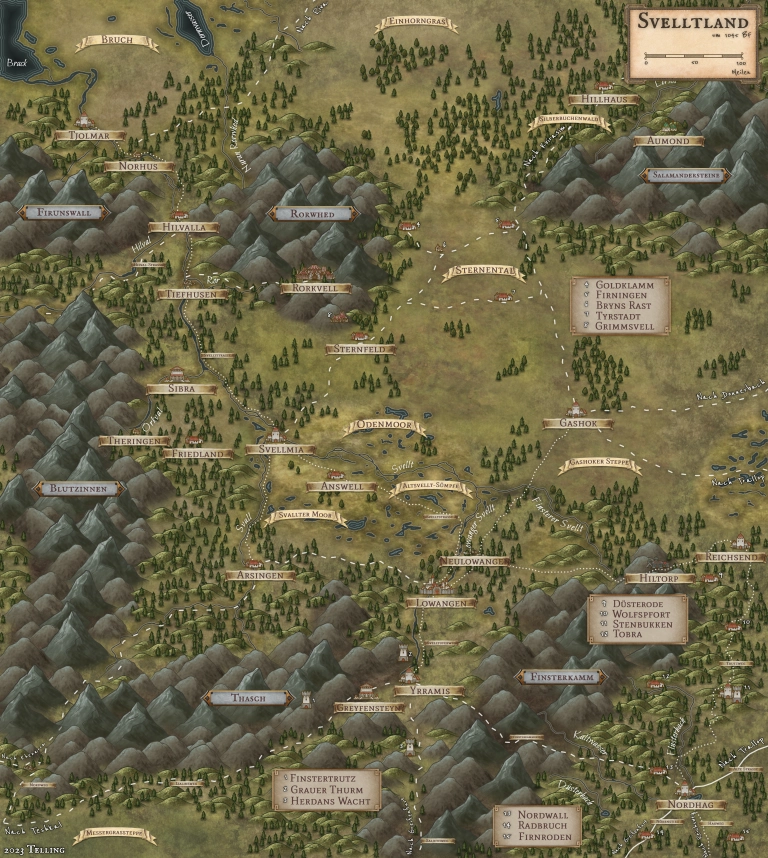
\includegraphics[width=\textwidth]{svellttal-0211.png}
\end{center}

\newpage

\spaltenanfang



\absatz{Tiere}
\label{svellt}
Die Tierwelt im Svelltland ist typisch für Nordaventurien und besonders von der Nähe zum \textbf{Orkland} geprägt,
welches Tieren wie \textbf{Orklandhörnchen} und \textbf{-karnickel} den Namen gegeben hat.
Dabei bietet das Land ganz unterschiedliche Lebensräume:
In Wiesen und Auen leben \textbf{Rebhühner}, \textbf{Rehe}, \textbf{Rotpüschel}, \textbf{Pfeifhasen} und \textbf{Steppenhunde}.
Am Fluss gibt es \textbf{Fischotter}, \textbf{Biber} und \textbf{Molche}. All diese Tiere können die Helden zu Gesicht bekommen, ohne die Straße zu verlassen. In den weiten Ebenen leben sogar \textbf{Nashörner} und \textbf{Mammuts}.
Zu den Raubtieren zählen vor allem die \textbf{Silberwölfe}, die nicht nur im Rorwhed auftreten. Nur selten sieht man auch \textbf{Rauwölfe} und \textbf{Orklandbären.}

Erst abseits der Straßen im Wald findet man \textbf{Wildschweine}, \textbf{Streifendachse}, \textbf{Auerhühner}, \textbf{Waldwölfe} und (seltener) \textbf{Waldlöwen}. Dazu kommen in den Gebirgen auch \textbf{Böcke}, \textbf{Murmeltiere} und die \textbf{Halmar-Antilope}.

\neuespalte

\absatz{Pflanzen}
Das Abenteuer spielt im Frühsommer, sodass sich viele örtlichen Pflanzenarten bereits zeigen und manche können auch schon geerntet werden. Entlang der Straßen und auf den Wiesen fallen darunter am häufigsten \textbf{Gulmond}, \textbf{Tarnele} und \textbf{Wirselkraut}, etwas seltener auch \textbf{Zwölfblatt}.

Am Waldrand hat man häufig Glück mit der \textbf{Vierblättrigen Einbeere}.

Nahe Flussufern und in Sümpfen wachsen \textbf{Donf}, \textbf{Roter Drachenschlund} und \textbf{Traschbart}.

\spaltenende
\neueseite
\spaltenanfang

\absatz{Kampfwerte}

\kreatur{Bandit}{Bandit}{humanoid}{
    \kreaturkampfwerte{4}{5}{4}{2}
    \trennlinie
    \kreaturvorteile{Zweihändig}
    \trennlinie
    \kreaturwaffe{Keule}{1}{8}{8}{2W6}{Kopflastig, stumpf}
}

\kreatur{Riesenamöbe}{Riesenamöbe}{tier}{
    \kreaturkampfwerte{6}{14}{1}{2}
    \trennlinie
    \kreaturvorteile{Körperlosigkeit, Schmerzimmun II}
    \trennlinie
    \kreaturwaffe{Scheinarm}{1}{2}{6}{1W6}{Ätzend (Ein Opfer in der Umklammerung erleidet in jeder INI-Phase 2W6 SP), 	Umklammern (-2, die Riesenamöbe kann nur ein Opfer umklammern)}
}


\absatz{NSCs}
\unterabsatz{Lowangen}
\begin{itemize}
    \item \textbf{Kontor Stoerrebrandt}
        \begin{itemize}
        	\item  Valpo Lucianus von Sturzbach, Sekretär von Vanjescha Stoerrebrandt, blonde Haare mit gezwirbelten Schnauzbart, immer nach neuester horasischer Mode gekleidet, Zwicker in der Westentasche
        \item Palla und Lothar -- Angestellte des Kontors, freundlich, aber diskret
                \end{itemize}
    \item \textbf{Straßenbande}
                \begin{itemize}
        	\item  Leon Winkelhauser -- Veteran der Ork-Belagerung von 1031 BF, hat zwei Finger während einer Attacke verloren, grimmiges Auftreten
        \item Praiosmine Algerein -- hat ihren Verlobten während der Belagerung verloren, hübsches Gesicht
        \item Raul Zerte -- albernischer Söldner, ist nur aus Solidarität dabei
        \item Neowen Inveric -- war zu jung, um selbst in der Belagerung zu kämpfen, verehrt aber bis heute die \enquote{Helden} von damals
    \item Quin Lonnert -- ehemaliger Schmuggler, hat zwei Töchter, die Mutter ist kurz vor der Belagerung an einem Fieber gestorben
    \item Hierosebia Damicilia Pantalogereon, ehemalige fahrende Medica und Quacksalberin, heute Besitzerin einer kleinen Apotheke in Lowangen, weiches Herz für Außenseiter
    \end{itemize}
    \item \textbf{Ordenshaus Graue Stäbe}
                \begin{itemize}
        	\item  Barngrimm Radobrecht, den Großmeister des Ordens der Grauen Stäbe in Lowangen, kurze dunkle Haare und Bart, sanfte Stimme, tatkräftig, bodenständig, Vorurteile gegen Orks
      \item  Magistra ordinaria Vistella Jolen, hat den Ascheregen als magisch erkannt, strenges Gesicht, glatte blonde Haare, die nach hinten gekämmt sind
        \item Meera, Luis und Götz -- Adepten der Grauen Stäbe, tauschen sich über den neuesten Tratsch ihrer Vorgesetzen aus -- auch wenn sie ernsthafte Schwierigkeiten bekommen würden, wenn diese je erfahren würden, dass ihre Untergebenen die Verschwiegenheitsklausel nicht sonderlich ernst nehmen.
        \end{itemize}
        \end{itemize}

\unterabsatz{Reise zum Rorwhed}
  \begin{itemize}
  	\item \textbf{Gasthaus}
                \begin{itemize}
        	\item  Der alte Strupp, sieht aus wie 90, arthritische Finger, kann aber noch gut erzählen
        \item Azzan (Ork), Gushrok (Ork), Kupunda, Gisbert und Koschrik -- begeisterte Zuhörer
        \end{itemize}
    \item \textbf{Niedergebranntes Gehöft}
                \begin{itemize}
        	\item Bauernpaar Arba und Bredo Wollweber
        	\end{itemize}
\end{itemize}

\unterabsatz{Rorwhed}
     \begin{itemize}
   	\item \textbf{Hexenzirkel}
                \begin{itemize}
        	\item  Xerinn, eigeborene Schöne der Nacht, Oberhexe des Rorwhed-Zirkels, aufbrausend und kontrollierend, wallende rote Haare und katzengrüne Augen
       \item Bringimox, Mitglied der Verschwiegenen Schwesternschaft, Oberhexer des Grauen Waldes, berechnend, aber sanftmütig, weiße Haare, haselnussbraune Augen, überraschend muskulös für sein Alter
        \item Alvina, Schlangenhexe, dunkle Haare, tiefblaue Augen
        \end{itemize}
    \item \textbf{Goblins}
                \begin{itemize}
        	\item  Schamanin Aschka, die Verhüllte, ältere Goblinfrau, geduldig, aber vorsichtig, Vorurteil gegen bunt gekleidete Figuren
        \item Jägertrupp: Wassel, Broggo, Juulka und Frikka -- aufgeregte Jäger, die von der Schamanin den Auftrag erhalten haben, die Wildschweinfässer zu fangen
        \end{itemize}
    \item \textbf{Menschlich-orkische Jägergruppen}
            \begin{itemize}
    	\item Herdlind Silkwies -- wettergegerbte Jägerin, silberne Haare
        \item Avon Mühlenfels -- Spezialist für Wildschweinjagd, dicker Pelzmantel
        \item Sequin Winterkalt -- junger Rotschopf, trägt einen Fuchsschädel als Glücksbringer am Gürtel
        \item Korobai Felsvater, stoischer älterer Burrkuzk-Ork, guter Fallensteller
        \item Grashok Drachenschelle, reizbarer Burrkuzk-Ork, soll einen Drachen geohrfeigt haben
        \end{itemize}
    \item \textbf{Dryade Venaya}, etwas größer als Menschen, 
    \end{itemize}

\info{
    \absatz{Generische Namen}
    \textbf{weiblich:}
    Dramina Gesse, Glenna Fassmacherin, Ilke Gerrholt, Traute Netzknüpferin \\
    \textbf{männlich:}
    Drego Rastburger, Elfwyn Kevendoch, Irian Dinckel, Gerding Linnenschneider
}

\spaltenende

\kasten{
\absatz{Quelle 1: Augenzeugenbericht}
\label{aiw_quelle1}
\enquote{Der Angriff hat nachts stattgefunden.
	Es schien plötzlich noch dunkler zu werden und ein Rauchgeruch hing in der Luft, der nicht von unserem kleinen Feuer stammen konnte.
	Beißender Qualm hat einen nach dem anderen zum Husten gebracht und die Sicht war schlecht. Die Gestalt, die dann aufgetaucht ist, schien geradewegs vom Himmel auf uns herabzufahren und aus Rauch und Qualm zu bestehen. Um sie herum begann das Gras zu schwelen und zu verkohlen. Wir leisteten kurz Widerstand, konnten aber gegen die allgegenwärtige Hitze nicht lange ankommen, zumal uns das Atmen schwer fiel. Inmitten des dichtesten Qualms habe ich aber eine etwa menschengroße Gestalt ausmachen können, die mich an ein Zündholz erinnert hat oder an eine halb erstickte Fackel, denn sie war dünn und verkohlt. Halb geblendet und nach Luft ringend sind alle in die Nacht geflohen, jeder in eine andere Richtung. Als ich an den Fluss kam, konnte ich mich dort im Dickicht am Ufer verbergen und mir den ganzen Ruß abwaschen. Noch am nächsten Morgen brannten mir die Augen.}
}

\absatz{Quelle 2: Die Weinlegende}
\label{aiw_quelle2}
Ihr betretet eine Holzhütte, die aussieht, als wäre sie vor kurzem aus frischen Buchenholz zusammengeschustert worden und die euch als Gasthaus beschrieben wurde. Innendrin entdeckt ihr einen schummrigen Saal mit vielen langen Tafeln und ihr seid erleichtert, dass der Duft des frischen Holzes noch nicht von diversen anderen Gerüchen jahrelangen Tavernenbetriebes überlagert wird.

Nur die bunt zusammengewürfelte Gruppe von Berufs- und Hobbytrinkern stört das würzige Aroma des hellen Schankraumes.
Diese hat sich in der Nähe des Tresens um einen älteren Gesellen mit roter Nase versammelt, dem gerade ein neues Glas Schnaps eingeschenkt wird.

\enquote{Wo war ich?}, stammelt der Alte.\\
\enquote{Bei Jokmanns Wein, Opa}, erklärt einer der Männer ungeduldig.\\
\enquote{Ach ja. Also das war damals so: Wie ich schon sagte, hatte der alte Jokmann das Jagen schon halb aufgegeben, weil das Revier, das er damals vom alten Firnwulf geerbt hatte, von dem alten Gierschlund so richtig ratzekahl leergejagt worden ist. Da hattest du vielleicht höchstens eine einzige Wildschweinrotte mit 10 Tieren, die Hälfte davon waren Frischlinge, alle noch an Mutterns Zitze und die andere Hälfte war so alt und zäh, die hätte nicht mal unser guter Alrik hier weichgeschmort bekommen.\\	
Der Rest vom Wild hatte sich komplett drüben zu den Hexen verdrückt, weil die nix dagegen hatten, dass die die ganzen Jungtriebe von den Tannen abknabbern. Aber wenn du die das machen lässt, dann hast du ruckzuck den ganzen Wald kaputt und dann ist gar nix mehr mit jagen, das sag ich dir!

Na ja, wie ich sagte, Jokmann war ziemlich am Ende. Und dann sagte er sich:
\enquote{Komm, einen letzten Ausflug machst du noch und wenn Firun dann nicht mit dir ist, dann gehst du zurück in die Stadt und suchst dir eine Anstellung bei einem Bogenbauer oder beim Jagdvogt oder so.}
Also schnappt er sich seinen treuen Hund Pix und marschiert in die Wildnis. Wir dachten damals ja, den sehen wir nie wieder, ich mein, wir waren damals ja auch nur kleine Stöpsel und der hatte so einen grimmigen Gesichtsausdruck. Und dann kam eine Woche später auch noch ein Sturm auf und keine Spur von Jokmann! Aber als wir schon alle Hoffnung aufgeben wollten, stapft der plötzlich in einer Vollmondnacht in den alten Gasthof und ihr glaubt nicht, wie der aussah! Nix mit dem schmucken Ledermantel, den er anhatte, als er losging, nein! Einen Wildschweinpelz trug er, mit so farbigen Verzierungen drauf und der roch! Der halbe Schankraum hat ihn angestarrt, als wäre er aus Borons Hallen selbst entwischt, gesegnet sei der Rabe.}

Ihr merkt wie die Spannung unter den Zuhörern steigt. Lange kann es nicht mehr dauern, bis die Geschichte ihrem Höhepunkt zustrebt.\\
\enquote{Na ja, dann waren natürlich alle erst mal heilfroh, dass Jokmann noch da war, vor allem, als man gemerkt hat, dass da immer noch der alte Halunke unter dem Pelz steckt. Den Hund hat er auch wieder mitgebracht und der sah auch aus, als hätte den jemand angemalt. Komisch wurde die Sache aber erst in den Wochen danach. Der ist nämlich dann nicht in die Stadt gegangen für eine Anstellung, nein, der ist im Jagdrevier vom alten Firnwulf geblieben. Der hat sogar die anderen zu einer Drückjagd eingeladen, weil er da den prächtigsten Hirsch gesehen haben wollte, den Tsa jemals auf Dere geschickt haben soll. Die einzige Bedingung war, dass sie alle vorher mit ihm diesen Wein trinken mussten, sonst würde die Jagd schiefgehen.}

Ihr könnt schwören, Opas Zuhörer halten den Atem an. Einer hüstelt kurz, worauf ihn alle anzischen.
\enquote{Das war ein seltsames Gesöff. Schmeckte fast wie Heidelbeerwein, aber irgendwie fad und erdig. Ich musste es einmal trinken, als sie mich bei einer Jagd als Treiber mitgenommen haben. Ist sofort in die Birne gestiegen und am Ende hab ich mein Mittagessen wieder ausgekotzt. Und die Flasche in der das war, ich will nicht wissen, wo die schon alles gewesen ist. Das war so eine raue Tonkaraffe mit ganz seltsamen Bildchen drauf, so Schweine und kleine Männchen mit Speeren.
	
Na ja, Jokmann hat halt alle dazu gedrängt, das Zeug zu trinken und los. Und tatsächlich sind die nach sieben Stunden mit einer fetten Hirschkuh als Beute zurückgekommen und die Leute haben noch Tage danach davon geschwärmt, dass der Hirsch, der die Kühe begleitet habe, der größte gewesen sei, den sie je gesehen hätten. Der bekam mit jedem Mal erzählen mehr Enden an seinem Geweih, ich sag's euch! 

Ja, und seitdem hatte der alte Jokmann nie wieder Pech beim Jagen, so lange er diesen Wein hatte. Und jedes mal, wenn wir dachten, die Flasche muss doch jetzt mal leer sein, ist der wieder für eine Woche im Wald verschwunden und dann war die wieder voll. Und bis zu seinem Todestag hat er dicht gehalten, wo er diesen Wein her hatte! Obwohl sich alle die Mäuler darüber zerrissen haben, mit Feenhügeln und Dämonenpakten und sonst noch was. Nie hat der was durchschlüpfen lassen! So, das ist jetzt die ganze Geschichte, jetzt gib mir mal was zu trinken, meine Kehle ist ja schon ganz trocken!}

Nachdem das Glas eilig aufgefüllt wurde, breitete sich Gemurmel in der Schankstube aus.
\enquote{Ob diese wandernden Fässer im Wald mit Jokmanns legendärem Wein zu tun haben?}\\
\enquote{Irgendetwas muss es damit auf sich haben, warum sonst sollte die Torfkompagnie eine Belohnung auf die Fässer ausgerufen haben?}



\absatz{Eigenheiten der Archetypen}

\spaltenanfang

\kreatur{Eisen-Ala}{}{humanoid}{
    \kreaturinfo{Düstere Vergangenheit}{Einen Teil ihrer Kampfausbildung verdankt sie ihrer Jugend bei den Schwarzamazonen. Zwar hat sie diesen Zeiten längst den Rücken gekehrt, doch beherrscht sie noch einige schmutzige Tricks und Techniken, die nicht als sonderlich rondragefällig gelten können. In vielen Regionen muss sie ihre Vergangenheit geheim halten.}
    \trennlinie
    \kreaturinfo{Von Rang und Namen}{Als Kriegerin wird sie hochgeschätzt und sie hat gelernt, sich entsprechend zu verhalten. Doch ihr Kriegerbrief ist in Wahrheit eine Fälschung.}
}
\kreatur{Falkja}{}{humanoid}{
    \kreaturinfo{Im Dienste der Schwänin}{Sie hat ihr Leben Ifirn geweiht und befolgt ihre Gebote.}
    \trennlinie
    \kreaturinfo{Meine Heimat - die Weite}{Sie hat den Großteil ihres Lebens in den Weiten des Nordens verbracht. Große Städte sind ihr schnell zu eng und mit Kälte kann sie besser umgehen als mit Hitze.}
    \trennlinie
    \kreaturinfo{Brückenbauen}{Sie strebt danach, Brücken zwischen den Elfen und den Zwölfgötter-Anhängern zu schlagen, die oft getrennte Gemeinschaften sind.}
}
\kreatur{Melcher}{}{humanoid}{
    \kreaturinfo{Kein Ekel, aber ekelig}{Er hat keine Scheu, sich alles anzusehen oder etwas anzufassen -- kommt gut mit Schmutz klar,  wirkt aber auch etwas ranzig.}
    \trennlinie
    \kreaturinfo{Tiere sind die besseren Menschen}{Er kommt einfach besser mit Tieren aus.}
    \trennlinie
    \kreaturinfo{Netter Kauz}{Man traut ihm zu, über manche speziellen Themen Bescheid zu wissen -- aber sicher nicht über alles. Sympathischer Typ, aber ein bisschen verrückt.}
}

\kreatur{Roana}{}{humanoid}{
    \kreaturinfo{Nebulöser Charakter}{Sie wirkt mysteriös und manchmal unauffällig, aber auch nicht immer sonderlich vertrauenswürdig -- besonders auf abergläubische Leute.}
    \trennlinie
    \kreaturinfo{Vergisst nie ein Gesicht}{Sie erkennt Leute immer wieder, doch ist dabei auch nachtragend und rachsüchtig.}
    \trennlinie
    \kreaturinfo{Wirren des Geistes}{Sie ist manchmal etwas verwirrt \dots in diesem Zustand kann sie leichter mit Geistern in Kontakt treten. Das mag zwar helfen, um diese zu bannen, führt aber manchmal im Gegenteil dazu, dass sie umso leichter einer Besessenheit erliegt.}
}

\kreatur{Wiesel-Rupo}{}{humanoid}{
    \kreaturinfo{Kennt keine Furcht\dots und keine Vernunft}{Er nimmt nichts wirklich ernst und alles auf die leichte Schulter und schätzt deshalb Risiken kaum ab. Mutproben sind oft erleichtert, aber er macht auch sehr riskante Sachen.}
    \trennlinie
    \kreaturinfo{Da gibt es doch ein Mittelchen}{Der Glaube des Charakters an die Wunder der Medizin ist stark ausgeprägt. Er hat selbst von eigentlich schlechten oder gar völlig unwirksamen Mitteln einen Placebo-Effekt und regeneriert eine Wunde oder einen Erschöpfungspunkt zusätzlich, doch wird dementsprechend beim Angebot jedes Quacksalbers schwach.}
    \trennlinie
    \kreaturinfo{Die Wahrheit wäre auch zu langweilig}{Er neigt zu Übertreibungen und schindet damit bei einigen ordentlich Eindruck, bei anderen eher das Gegenteil.}
    \trennlinie
    \kreaturinfo{Die kriegen mich eh nie}{Er muss geradezu zwanghaft am Tatort sein Markenzeichen zurücklassen - ein kleines Papier mit Schlangensymbol in die leere Hosentasche stecken oder in der leeren Schatztruhe platzieren. Wenn er das macht, ist sein Entkommen einfacher: Schleichen oder Klettern wird etwas erleichtert.}
}

\spaltenende